% Report 6 contribution: Nguyen Lu Nhat Huy (CE181196).
% Match the common Report6 preamble; no additional packages required.
\newpage
\subsection{Identity Verification and Expert Workspace}

\subsubsection{M5.01 -- Submit Identity Verification}
\begin{itemize}[leftmargin=1.5em,itemsep=2pt]
  \item \textbf{Screen Name \& Route Path:}\newline \texttt{/freelancer/profile?tab=identity or /client/profile?tab=identity}.
  \item \textbf{Target Actor:} Freelancer or Client.
  \item \textbf{Preconditions:} Signed in; readable document images and a working webcam are available.
  \item \textbf{Purpose:} Submit document images and live face evidence for identity verification.
\end{itemize}
\paragraph{Screen-Transition Workflow:} Identity $\rightarrow$ document type and images $\rightarrow$ liveness challenge $\rightarrow$ Submit for AI verification $\rightarrow$ status.
\begin{figure}[H]\centering
\scalebox{0.5114}{%
\begingroup\setlength{\unitlength}{1pt}\linethickness{0.9pt}
\begin{picture}(450.00,254.21)
\put(0,0){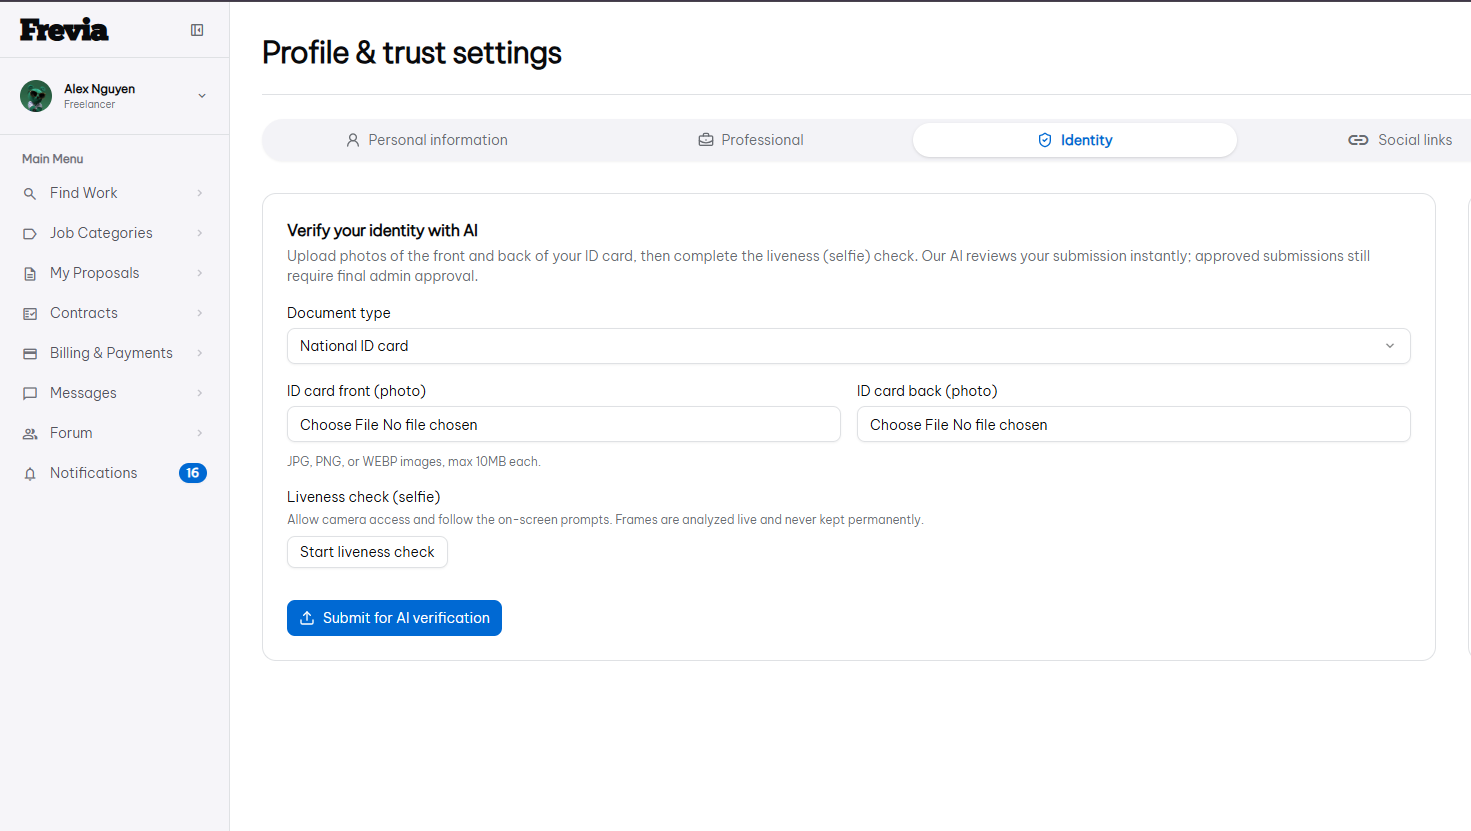
\includegraphics[width=450.00pt]{images/freelancer/m5_01_upload_identity_documents.png}}
\put(87.30,116.94){\color{fptred}\framebox(344.70,15.25){}}
\put(87.30,132.19){\colorbox{white}{\textcolor{fptred}{\scriptsize\bfseries 1}}}
\put(87.30,79.57){\color{fptred}\framebox(50.40,11.95){}}
\put(87.30,91.52){\colorbox{white}{\textcolor{fptred}{\scriptsize\bfseries 2}}}
\put(87.30,58.47){\color{fptred}\framebox(67.50,12.71){}}
\put(87.30,71.18){\colorbox{white}{\textcolor{fptred}{\scriptsize\bfseries 3}}}
\end{picture}
\endgroup}%

\caption{Identity form: document images, liveness check and submission.}
\label{fig:r6_m5_01_upload_identity_documents}
\end{figure}
\paragraph{Step-by-Step User Instructions:}
\begin{enumerate}[leftmargin=1.8em,itemsep=3pt]
  \item \rbadge{1} Open Identity and select the appropriate Document type.
  \item \rbadge{2} Choose the front image and, when appropriate for the document, its back image. The form accepts JPG, PNG and WebP; each document image must be no larger than 10 MB.
  \item \rbadge{3} Allow browser camera access and select Start liveness check. Follow the on-screen challenge until capture completes; the first captured frame supplies the selfie.
  \item \rbadge{4} Select Submit for AI verification once. Keep the page open while verification is running.
  \item \rbadge{5} Read the resulting status and explanation. An AI-accepted submission still requires Administrator review.
\end{enumerate}
\paragraph{Expected Output \& Exception Handling:}
\begin{itemize}[leftmargin=1.5em,itemsep=2pt]
  \item \textbf{Expected result:} An AI-accepted submission is Pending for Administrator approval. An AI-rejected submission shows Rejected with the available reason.
  \item \textbf{Troubleshooting:} A front image and completed liveness capture are required. For camera errors, enable browser camera permission and retry the challenge.
  \item \textbf{Troubleshooting:} If the AI service or network fails, retry after it is restored. A transport error is not a successful submission. Already approved identity records cannot simply be resubmitted.
\end{itemize}

\newpage
\subsubsection{M5.02 -- View Identity Verification Status}
\begin{itemize}[leftmargin=1.5em,itemsep=2pt]
  \item \textbf{Screen Name \& Route Path:}\newline \texttt{/freelancer/profile?tab=identity or /client/profile?tab=identity}.
  \item \textbf{Target Actor:} Freelancer or Client.
  \item \textbf{Preconditions:} Signed in; a submission may or may not exist.
  \item \textbf{Purpose:} Check verification progress and review feedback.
\end{itemize}
\paragraph{Screen-Transition Workflow:} Identity $\rightarrow$ Verification status $\rightarrow$ Pending, Approved, Rejected or no submission.
\begin{figure}[H]\centering
\scalebox{0.9556}{%
\begingroup\setlength{\unitlength}{1pt}\linethickness{0.9pt}
\begin{picture}(450.00,195.57)
\put(0,0){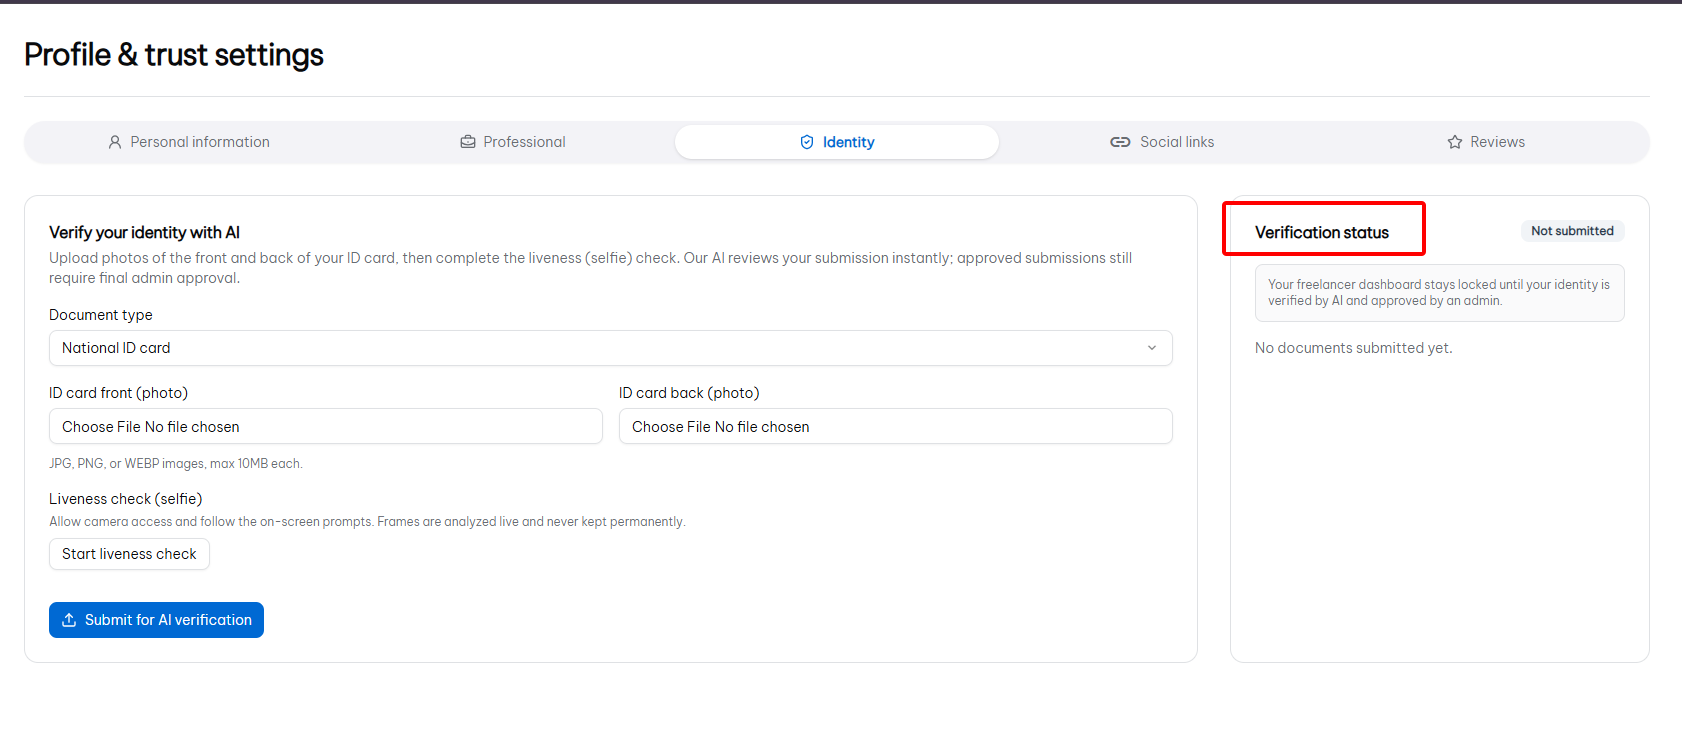
\includegraphics[width=450.00pt]{images/freelancer/m5_02_view_verification_status.png}}
\put(328.50,19.56){\color{fptred}\framebox(112.50,123.21){}}
\put(328.50,142.77){\colorbox{white}{\textcolor{fptred}{\scriptsize\bfseries 1}}}
\end{picture}
\endgroup}%

\caption{Verification status panel beside the submission form.}
\label{fig:r6_m5_02_view_verification_status}
\end{figure}
\paragraph{Step-by-Step User Instructions:}
\begin{enumerate}[leftmargin=1.8em,itemsep=3pt]
  \item \rbadge{1} Open Identity and read the Verification status panel.
  \item \rbadge{2} If Pending, wait for Administrator review. If Approved, use the account normally within its permissions.
  \item \rbadge{3} If Rejected, read the review notes and correct the underlying issue before starting another allowed submission.
\end{enumerate}
\paragraph{Expected Output \& Exception Handling:}
\begin{itemize}[leftmargin=1.5em,itemsep=2pt]
  \item \textbf{Expected result:} The panel shows the current stored verification status and any available review notes.
  \item \textbf{Troubleshooting:} No submission means no document record is displayed; it is not an approval. Refresh after a review decision. A rejected identity and a rejected profile revision are different records.
\end{itemize}


\newpage
\subsubsection{M13.01 -- Open Expert Workspace in Admin User Management}
\begin{itemize}[leftmargin=1.5em,itemsep=2pt]
  \item \textbf{Screen Name \& Route Path:}\newline \texttt{/admin/users?role=EXPERT}.
  \item \textbf{Target Actor:} Administrator or an internal user with user-management permissions.
  \item \textbf{Preconditions:} Signed in to the Admin Portal with permission to list and inspect users.
  \item \textbf{Purpose:} Locate Expert accounts in the shared User Management workspace.
\end{itemize}
\paragraph{Screen-Transition Workflow:} Admin Portal $\rightarrow$ Users $\rightarrow$ User Management $\rightarrow$ Filter Role: Expert $\rightarrow$ View details.
\begin{figure}[H]\centering
\scalebox{0.75962}{%
\begingroup\setlength{\unitlength}{1pt}\linethickness{0.9pt}
\begin{picture}(450.00,223.80)
\put(0,0){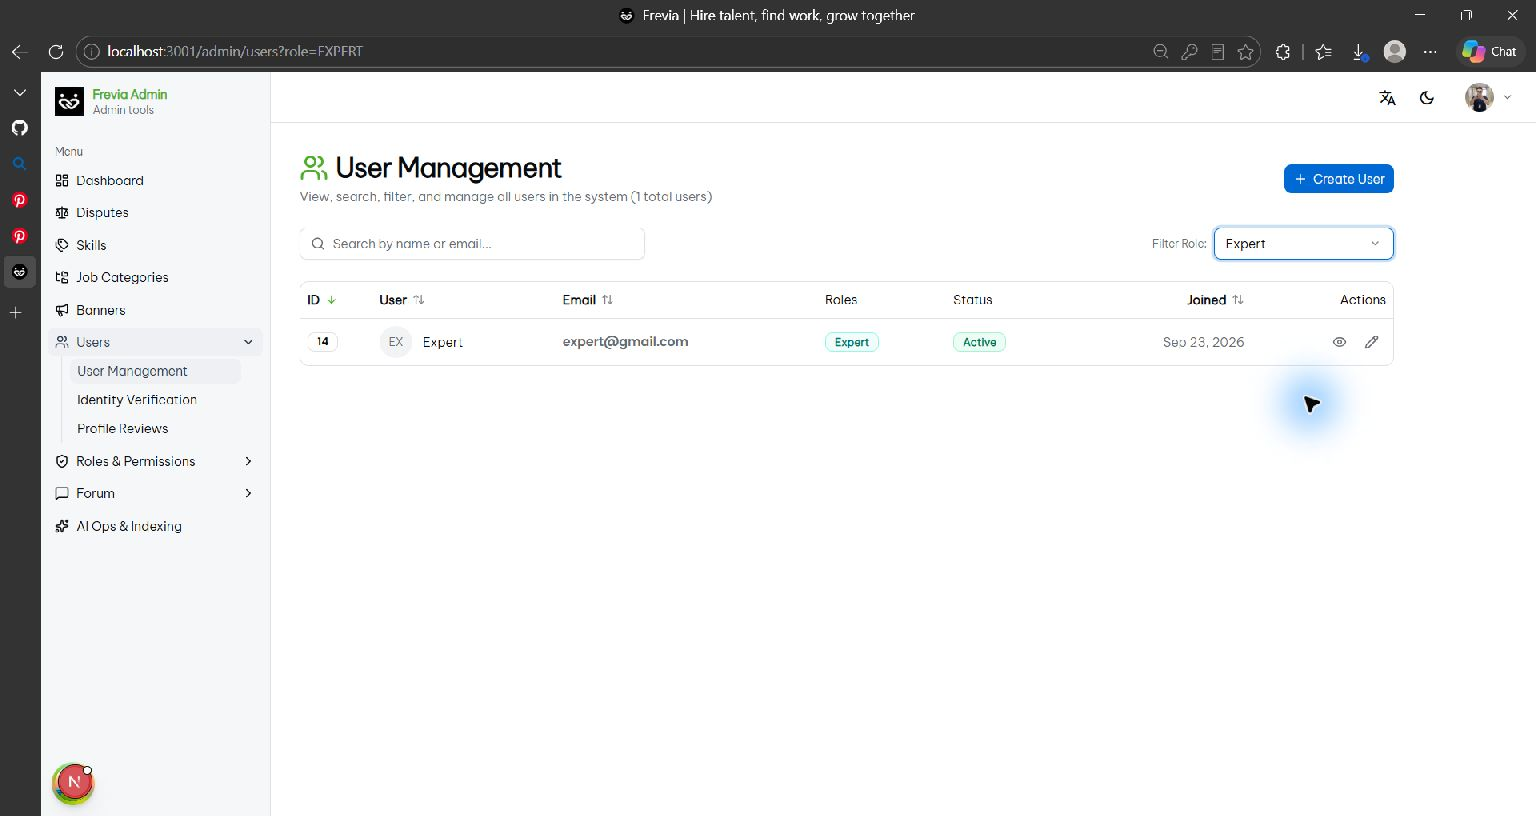
\includegraphics[width=450.00pt,trim=40bp 0bp 0bp 72bp,clip]{images/expert/m13_01_expert_user_management.png}}
\put(351.94,166.64){\color{fptred}\framebox(56.25,11.43){}}
\put(351.94,178.07){\colorbox{white}{\textcolor{fptred}{\scriptsize\bfseries 1}}}
\put(387.73,138.67){\color{fptred}\framebox(7.22,7.82){}}
\put(387.73,146.49){\colorbox{white}{\textcolor{fptred}{\scriptsize\bfseries 2}}}
\end{picture}
\endgroup}%
\caption{User Management filtered to Expert accounts; the eye action opens the selected user.}
\label{fig:r6_m13_01_expert_user_management}
\end{figure}

\paragraph{Step-by-Step User Instructions:}
\begin{enumerate}[leftmargin=1.8em,itemsep=3pt]
  \item \rbadge{1} In the Admin sidebar, expand Users and select User Management. Set Filter Role to Expert; use the name/email search if needed.
  \item \rbadge{2} Identify the intended Expert by name, email and role, then select its View details (eye) action.
  \item Inspect Role Profiles \& Granted Privileges and the Expert Profile tab. Expert dispute operations remain in the separately authorized Disputes area.
\end{enumerate}
\paragraph{Expected Output \& Exception Handling:}
\begin{itemize}[leftmargin=1.5em,itemsep=2pt]
  \item \textbf{Expected result:} The list contains matching Expert accounts and opens the selected account detail.
  \item \textbf{Troubleshooting:} Clear the search if no matches appear. Expert role membership alone does not grant permission to manage other users. This is the shared Admin workspace, not a separate \texttt{/expert} page.
\end{itemize}

\newpage
\subsubsection{M13.02 -- Maintain Expert Profile in User Management}
\begin{itemize}[leftmargin=1.5em,itemsep=2pt]
  \item \textbf{Screen Name \& Route Path:}\newline Expert Profile tab at \texttt{/admin/users/[id]}.
  \item \textbf{Target Actor:} Administrator or an internal user authorized to update Expert profiles.
  \item \textbf{Preconditions:} The intended Expert account is open; Expert-profile update permission is granted.
  \item \textbf{Purpose:} Maintain the Expert's professional information through the shared Admin editor.
\end{itemize}
\paragraph{Screen-Transition Workflow:} User Management $\rightarrow$ Expert details $\rightarrow$ Expert Profile $\rightarrow$ Edit profile $\rightarrow$ Save changes or Cancel.
\begin{figure}[H]\centering
\begin{minipage}[c]{0.48\textwidth}\centering
\scalebox{0.46918}{%
\begingroup\setlength{\unitlength}{1pt}\linethickness{0.9pt}
\begin{picture}(450.00,223.80)
\put(0,0){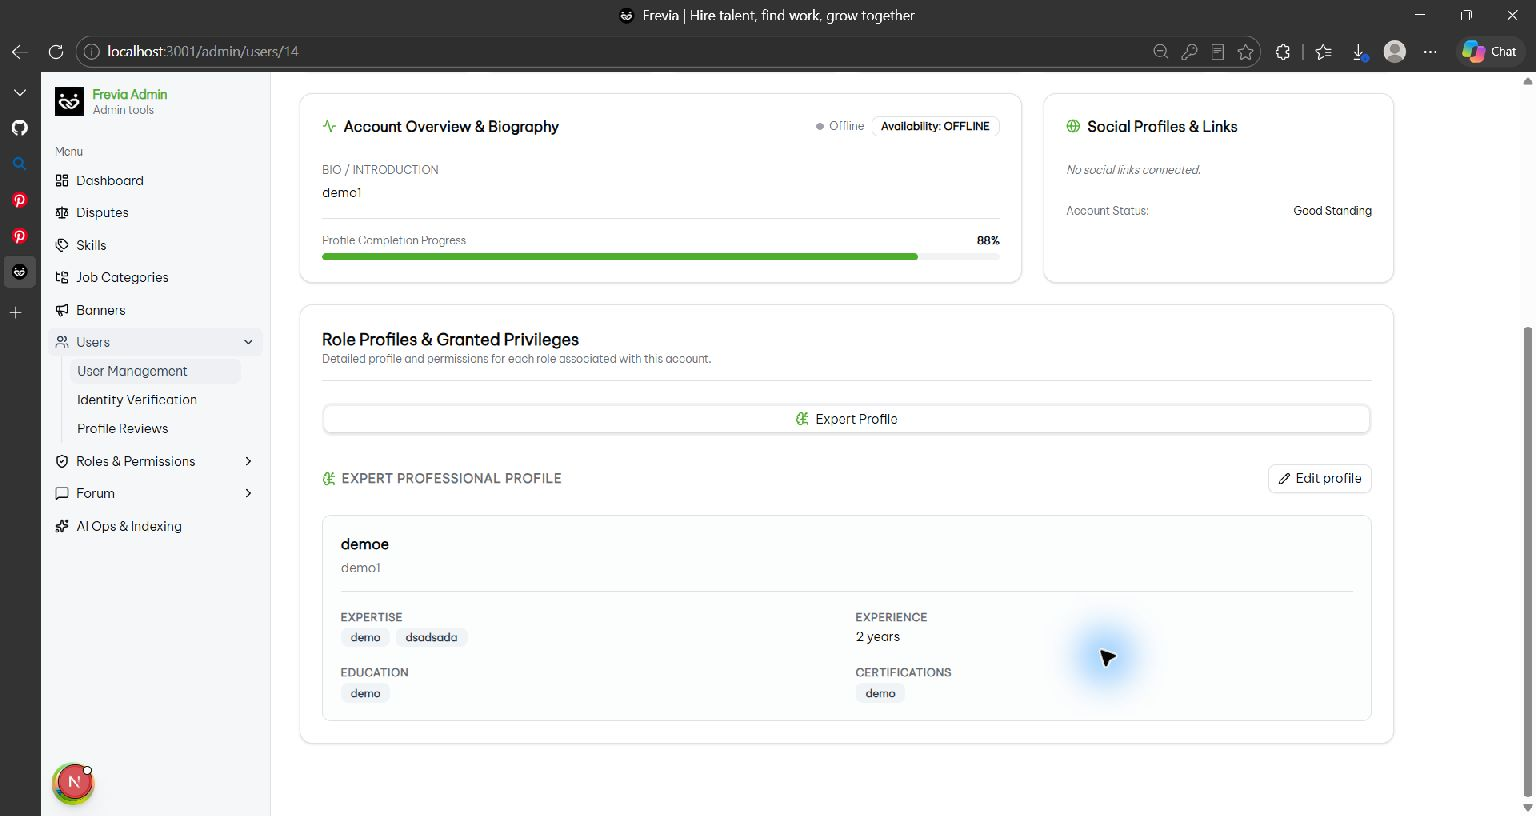
\includegraphics[width=450.00pt,trim=40bp 0bp 0bp 72bp,clip]{images/expert/m13_02_expert_user_detail.png}}
\put(368.48,96.26){\color{fptred}\framebox(33.09,10.23){}}
\put(368.48,106.48){\colorbox{white}{\textcolor{fptred}{\scriptsize\bfseries 1}}}
\end{picture}
\endgroup}%
\end{minipage}\hfill
\begin{minipage}[c]{0.48\textwidth}\centering
\scalebox{0.46918}{%
\begingroup\setlength{\unitlength}{1pt}\linethickness{0.9pt}
\begin{picture}(450.00,223.80)
\put(0,0){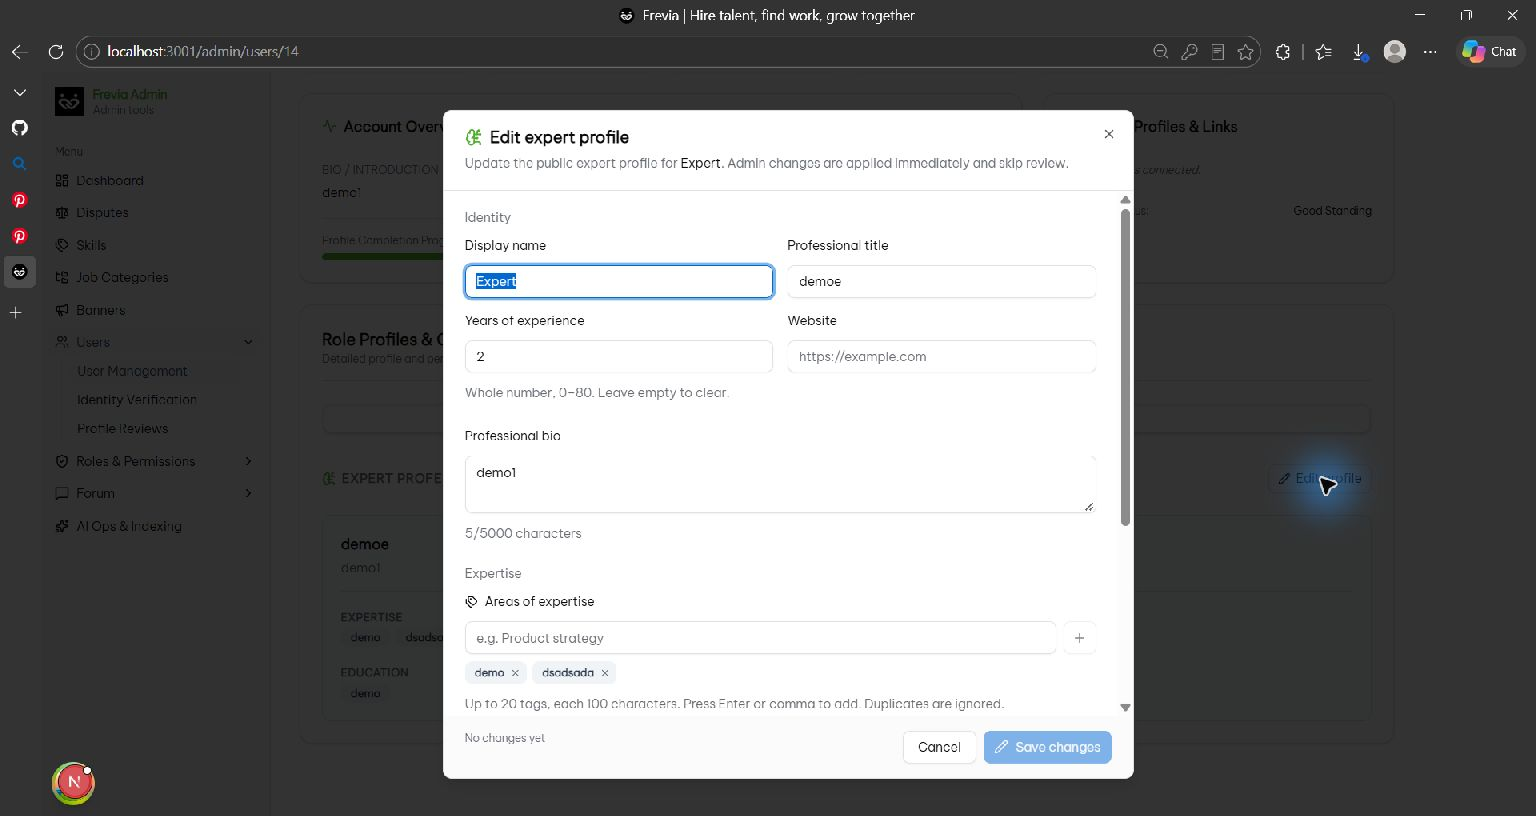
\includegraphics[width=450.00pt,trim=40bp 0bp 0bp 72bp,clip]{images/expert/m13_02_edit_expert_profile.png}}
\put(127.24,85.43){\color{fptred}\framebox(191.91,88.74){}}
\put(127.24,174.16){\colorbox{white}{\textcolor{fptred}{\scriptsize\bfseries 1}}}
\put(127.24,32.49){\color{fptred}\framebox(191.91,40.91){}}
\put(127.24,73.40){\colorbox{white}{\textcolor{fptred}{\scriptsize\bfseries 2}}}
\end{picture}
\endgroup}%
\end{minipage}
\caption{Expert Profile and Edit profile action (left); current Expert profile editor (right).}
\label{fig:r6_expert_profile_editor}
\end{figure}

\paragraph{Step-by-Step User Instructions:}
\begin{enumerate}[leftmargin=1.8em,itemsep=3pt]
  \item Select Expert Profile under Role Profiles \& Granted Privileges, then click Edit profile.
  \item Update Display name, Professional title, Years of experience, Website and Professional bio as required. Years must be a whole number from 0 to 80; bio supports up to 5000 characters.
  \item In Areas of expertise, add a tag using Enter or comma. Up to 20 tags of 100 characters each are supported; duplicates are ignored.
  \item Scroll inside the dialog to Education and Certifications. Use Add entry and the remove actions to maintain the lists. Check Directory visibility before saving.
  \item Select Save changes to apply the edit, or Cancel to leave the stored profile unchanged. Save changes is disabled until the form has changes.
\end{enumerate}
\paragraph{Expected Output \& Exception Handling:}
\begin{itemize}[leftmargin=1.5em,itemsep=2pt]
  \item \textbf{Expected result:} Successful Admin edits apply immediately and skip profile review, as stated in the dialog.
  \item \textbf{Troubleshooting:} Correct validation errors and check update permission if the editor is unavailable. General settings for the signed-in internal user remain at \texttt{/admin/profile}.
\end{itemize}

\newpage
\subsubsection{M13.03 -- Check Expert Profile Status and Review Outcome}
\begin{itemize}[leftmargin=1.5em,itemsep=2pt]
  \item \textbf{Screen Name \& Route Path:}\newline Expert Profile editor at \texttt{/admin/users/[id]}; Profile Reviews for actual submitted revisions.
  \item \textbf{Target Actor:} Authorized Administrator or internal profile reviewer.
  \item \textbf{Preconditions:} The Expert account can be inspected; decision permissions are required for revision review.
  \item \textbf{Purpose:} Distinguish Expert profile activity from a pending profile-review decision.
\end{itemize}
\paragraph{Screen-Transition Workflow:} Expert user detail $\rightarrow$ Edit profile $\rightarrow$ Directory visibility; actual submitted revision $\rightarrow$ Profile Reviews $\rightarrow$ review outcome.
\begin{figure}[H]\centering
\scalebox{0.64791}{%
\begingroup\setlength{\unitlength}{1pt}\linethickness{0.9pt}
\begin{picture}(450.00,223.80)
\put(0,0){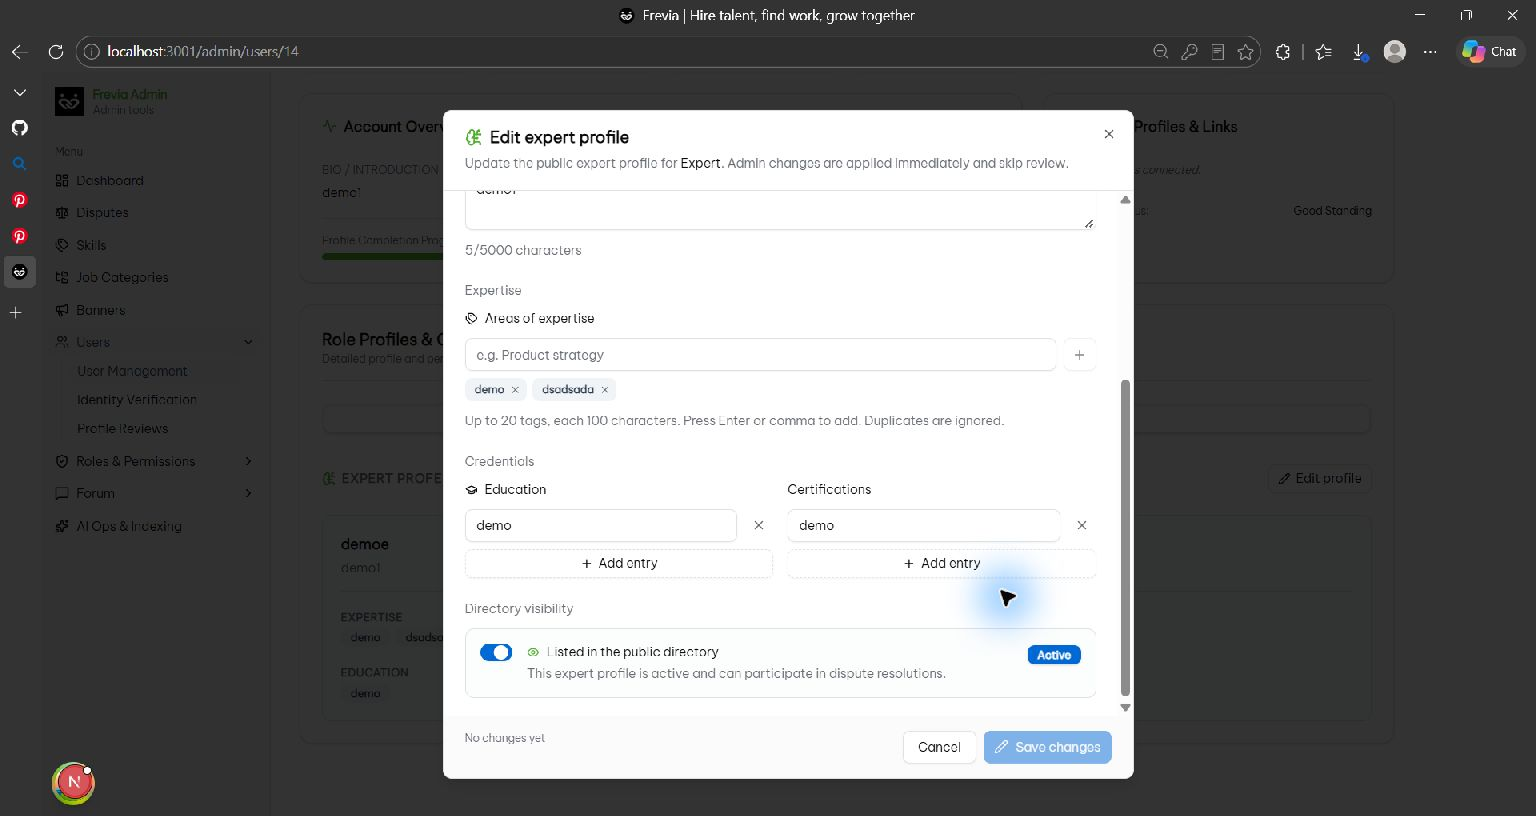
\includegraphics[width=450.00pt,trim=40bp 0bp 0bp 72bp,clip]{images/expert/m13_03_expert_credentials_status.png}}
\put(127.24,70.39){\color{fptred}\framebox(191.31,30.68){}}
\put(127.24,101.07){\colorbox{white}{\textcolor{fptred}{\scriptsize\bfseries 1}}}
\put(127.24,34.89){\color{fptred}\framebox(191.31,21.66){}}
\put(127.24,56.55){\colorbox{white}{\textcolor{fptred}{\scriptsize\bfseries 2}}}
\end{picture}
\endgroup}%
\caption{Expert credentials and Directory visibility in the current Admin editor.}
\label{fig:r6_m13_03_expert_credentials_status}
\end{figure}

\paragraph{Step-by-Step User Instructions:}
\begin{enumerate}[leftmargin=1.8em,itemsep=3pt]
  \item Inspect Directory visibility and its Active state. The current form explains that an active Expert profile can participate in dispute resolutions.
  \item Distinguish this profile state from the user account's Active/Banned status. It is also not a Pending/Approved/Rejected review decision.
  \item Admin edits made with M13.02 apply immediately and skip review. If a revision was submitted through a review-based flow, an authorized reviewer checks Profile Reviews under M16.02 and reads its decision/notes.
\end{enumerate}
\paragraph{Expected Output \& Exception Handling:}
\begin{itemize}[leftmargin=1.5em,itemsep=2pt]
  \item \textbf{Expected result:} The guide identifies the profile's current activity state without incorrectly treating every Admin edit as a pending submission.
  \item \textbf{Troubleshooting:} A visibility control labelled public directory does not establish that a public \texttt{/experts} page is available. No standalone Expert review-status page was observed in this workflow.
\end{itemize}
